\section{Infrared Thermography}

Infrared tomography is an imaging technique that utilizes infrared radiation emitted from nearly any objects. 
The existence of infrared radiation was first discovered in 1800 by Sir Frederick William Herschel. 
His experiments lead to the knowledge that there were a light spectrum beyond the visual spectrum humans are able to perceive.\cite{ignacio2017,optris2009}

Infrared thermography is commonly used to calculate surface temperatures and important concepts in the understanding of this are heat and temperature. 
Temperature is a measure for the internal energy within an object and can be defined at the average kinetic energy of the object.
Heat is the energy that passes from a warm object to another colder object. A warm object will decrease in internal energy and a cold object will increase due to the temperature difference and therefore the heat transfer. In the human body, a constant temperature is keep, due to several factors and therefore the temperature will not decrease even though a heat transfer to the surrounding environment occurs. The environmental temperature do have an impact on how large the heat transfer gradient is. If a body is in a cold environment, the emitted heat will be grater than the absorbed. In the same way, if the environment is much warmer than 37 degrees Celsius, a greater absorption than emission will occur and the body will increase in temperature.\cite{ignacio2017} 



\subsection{Physical principals}

Any object above absolute zero emits energy-electromagnetic radiation depending on its temperature. Absolute zero is $0$ Kelvin or $ -273.16 $ Celsius. To put that into perspective the human body has a temperature around 37 degrees Celsius.\cite{ignacio2017,optris2009}

Electromagnetic radiation is a propagation of energy trough a medium without the transportation of mass. An electromagnetic wave is made of the relationship between frequency (f), wavelength ($\lambda$) and the speed of light (c). This is stated in the equation of wave motion.\cite{ignacio2017}  
\begin{flalign}
	\lambda = \frac{c}{f}
	\label{eq:wave}
\end{flalign}
Depending on the frequency and wavelength certain characteristics arise from what is called the electromagnetic spectrum. The electromagnetic spectrum is the electromagnetic energy that is emitted. This extends from radiation of low energy such as radio waves and infrared, to waves of higher energy in form of eg. X-rays. A graphical representation of the electromagnetic spectrum can be seen on \cref{fig:em_spectrum}.\cite{ignacio2017}        

\begin{figure}[H]                                         
	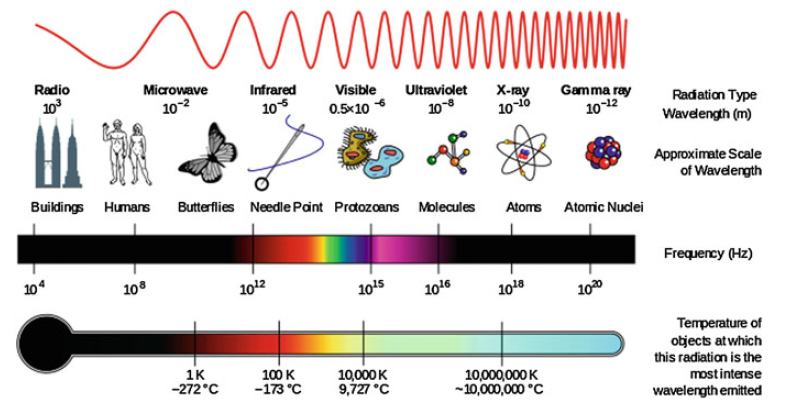
\includegraphics[width=.66\textwidth]{figures/em_spectrum}  
	\caption{The electromagnetic spectrum with wavelength, emitters, frequency and temperature.\cite{ignacio2017}}
	\label{fig:em_spectrum}  
\end{figure}   

Infrared radiation is also known as thermal radiation because the relationship between temperature and infrared radiation. Temperature of the human body permits radiation in the infrared spectrum, but objects of much higher temperature are capable of emitting radiation in the visible and UV spectrum. This has to do with the difference between object and environmental temperature. If the temperature of these are relatively close to each other, the radiation emitted will be within infrared wavelengths. Infrared radiation have a wavelength from 769nm to 1mm. Objects emit more radiation in some region regions compared to others. Because of this is the infrared spectrum classified in the three regions, near, middle and far infrared. Near is between 769nm and 2.5$\mu$m, middle 2.5$\mu$m to 50$\mu$m and far 50$\mu$m to 1mm. The human body emits most radiation in the far infrared part, and most thermal cameras are build with this in mind. Near and middle cameras are used to measure gases.\cite{ignacio2017} 



\subsection{Measuring thermal energy}

Measuring thermal radiation uses the knowledge that electromagnetic radiation is proportional to the internal energy. With a lens, the radiation beam emitted, is focused on to a detector element that generates an electric output proportional to the radiation.\cite{optris2009}

\begin{figure}[H]                                         
	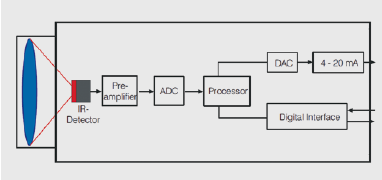
\includegraphics[width=.55\textwidth]{figures/IR_cam}  
	\caption{Simplified block diagram of an standard infrared camera.\cite{optris2009}}
	\label{fig:em_spectrum}  
\end{figure} 

extra notes that i'we just copied that we can use later 
The advantages of non-contact temperature measurement
are obvious – it supports:
• Temperature measurements of moving or overheated
objects and of objects in hazardous surroundings
• Very fast response and exposure times
• Non-interactive measurement, no influence on
the measuring object
• Non-destructive measurement
• Measurement point durability, no mechanical wear


